\documentclass[aspectratio=169]{beamer}

\usetheme{default}
\setbeamertemplate{navigation symbols}{}
\setbeamertemplate{enumerate item}{\color{navy}\arabic{enumi}.}
\setbeamertemplate{itemize item}{\color{black}\textbullet}
\setbeamertemplate{itemize subitem}{\color{black}\textbullet}
\usepackage{booktabs}
\usepackage{xcolor}
\usepackage{tikz}
\usetikzlibrary{shapes,arrows,positioning}
\definecolor{navy}{RGB}{0, 0, 128}
\definecolor{lightblue}{RGB}{230,240,250}
\definecolor{darkgreen}{RGB}{0,100,0}
\definecolor{lightgreen}{RGB}{230,250,230}
\newcommand{\highlight}[1]{\colorbox{lightblue}{$\displaystyle\textcolor{navy}{#1}$}}
\newcommand{\highlighttext}[1]{\colorbox{lightblue}{\textcolor{navy}{#1}}}
\newcommand{\highlightgreen}[1]{\colorbox{lightgreen}{$\displaystyle\textcolor{darkgreen}{#1}$}}

\begin{document}

\begin{frame}

Model fit consists of showing that your model can match the data

\bigskip{}

\onslide<2->{
\begin{itemize}
\itemsep1.5em
\item<2-> Counterfactuals rely solely on the model
\item<3-> Most model fit is \textit{ad hoc}: you can choose what to show
\item<4-> Typically, show that moments of $Y$ variables match
\item<5-> e.g. choice frequencies in data match choice probabilities of model
\item<6-> Other moments may be of interest, like dynamic choice transitions
\end{itemize}
}

\end{frame}

\begin{frame}
\centering
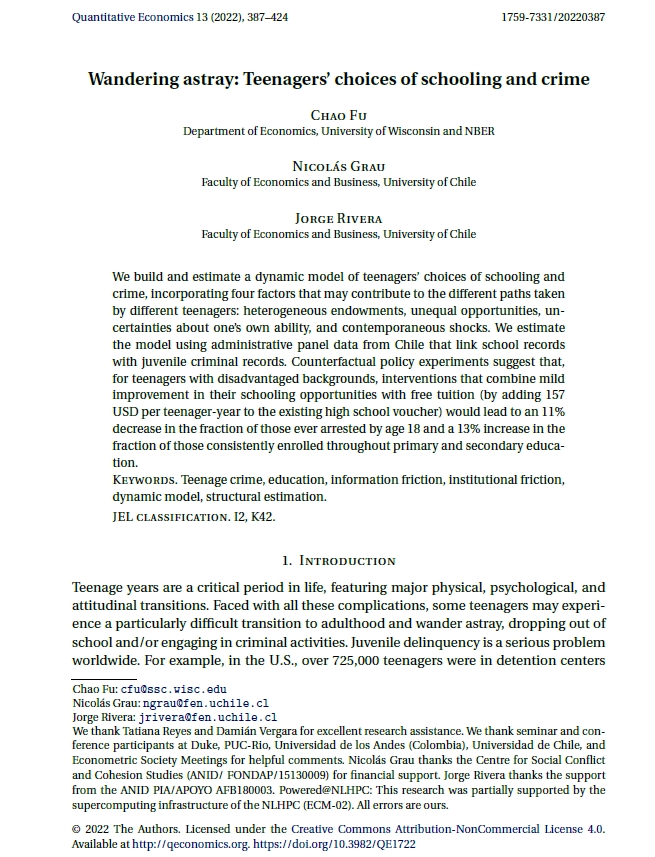
\includegraphics[width=0.4\textwidth]{Fu_al_cover.jpg}
    
\end{frame}


\begin{frame}

\onslide<1->{
Model fit results for youth with parents who are not well educated:

\bigskip{}

\begin{table}
\begin{tabular}{lcc}
\toprule
Variable & Data & Model \\
\midrule
Ever arrested \% & 5.6 & 5.2 \\
Always enrolled, 0 arrest \% & 72.2 & 72.0 \\
GPA (standardized) & -0.39 & -0.43 \\
Retention \% & 7.3 & 7.8 \\
Grade Completed by T & 11.1 & 11.3 \\
\bottomrule
\end{tabular}
\end{table}
}

\onslide<2->{
\bigskip{}
Model fit for other groups is similar
}

\end{frame}

\begin{frame}

Two options for producing model fit statistics:

\bigskip{}

\begin{itemize}
\itemsep1.5em
\item<2-> Use model assumptions and estimates to simulate a new dataset, $\tilde{Y}$ vs. $Y$
\item<3-> Use data and estimates to compute $\hat{Y}$ and compare with $Y$
\end{itemize}

\end{frame}

\begin{frame}

\textcolor{navy}{Option 1: Simulating a new dataset}

\bigskip{}

\begin{itemize}
\itemsep1.5em
\item<2-> Draw the unobservables from the model
\item<3-> Use any initial conditions from the data
\item<4-> If dynamic: draw $Y$ in $t=1$
\begin{itemize}
    \item<5->[]
    \item<5-> Update $X$'s in $t=2$ and draw $Y$ in $t=2$, and so on
\end{itemize}
\item<6-> If using SMM, you should already have code for this
\item<7-> Repeat process multiple times and take average to limit simulation error
\end{itemize}

\end{frame}

\begin{frame}

\textcolor{navy}{Option 2: Predict from data and estimates}

\bigskip{}

\begin{itemize}
\itemsep1.5em
\item<2-> Predict $\hat{Y}$ using the actual data
\item<3-> Identical to using a \texttt{predict()} function
\item<4-> May not be possible if model has key latent variables
\item<5-> e.g. unobserved types or other unobservables not in data
\item<6-> In such cases, must use simulation route
\end{itemize}

\end{frame}

\end{document}